\documentclass[12pt, a4paper]{article}

%%%%%%%%%%%%%%%% PACKAGES %%%%%%%%%%%%%%%%%%%%%

\usepackage[utf8]{inputenc}
\usepackage[english]{babel}

\usepackage{amsmath}
\usepackage{amsthm}
\usepackage{amssymb}
\usepackage{bm}
\newtheorem{theorem}{Theorem}[section]
\newtheorem{corollary}{Corollary}[theorem]
\newtheorem{lemma}[theorem]{Lemma}
\newenvironment{claim}[1]{\par\noindent\underline{Claim:}\space#1}{}
\newenvironment{claimproof}[1]{\par\noindent\underline{Proof:}\space#1}{\hfill $\blacksquare$}

\usepackage{hyperref}
\usepackage{parskip}
\usepackage{abstract}
\usepackage{tocbibind}

\usepackage{graphicx}
\graphicspath{{./images/}}

\usepackage[linesnumbered, vlined,ruled, commentsnumbered]{algorithm2e}
\usepackage{minted}
\newcommand{\code}[1]{\texttt{#1}}

\usepackage[acronym]{glossaries}

%%%%%%%%%%%%%%%% CONFIG %%%%%%%%%%%%%%%%%%%%%

\renewcommand{\absnamepos}{flushleft}
\setlength{\absleftindent}{0pt}
\setlength{\absrightindent}{0pt}


%%%%%%%%%%%%%%%% HEADER %%%%%%%%%%%%%%%%%%%%%

\usepackage{fancyhdr}
\pagestyle{fancy}
\fancyhf{}
\rhead{Arnau Abella}
\lhead{Algorithmics for Data Mining}
\rfoot{Page \thepage}

%%%%%%%%%%%%%%%% TITLE %%%%%%%%%%%%%%%%%%%%%

\title{%
  \textit{FP-growth} distilled
}
\author{%
  Arnau Abella \\
  \small{Universitat Polit\`ecnica de Catalunya}
}
\small{\date{\today}}

%%%%%%%%%%%%%%%% DOCUMENT %%%%%%%%%%%%%%%%%%%%%

\begin{document}

\maketitle

\section{Introduction}

Apriori-like candidate set generation-and-test approach is based on the \textit{anti-monotone Apriori heuristic: if any length k patterns is not frequent in the database, its length $k + 1$ super-pattern can never be frequent.} The essential idea is to iteratively generate the set of candidates patterns of length $k+1$ from the set of frequent-patterns of length $k$ (for $k \geq 1$), and check their corresponding ocurrence frequencies in the database.

The \textit{Apriori} heuristic achieves good performance gained by (possibly \\ significantly) reducing the size of candidate sets. However, in situations with a large number of frequent patterns, long patterns, or quite low minimum support thresholds, an \textit{Apriori}-like algorithm may suffer from the following: it is costly to handle a huge number of candidate sets. For example, if there are $10^4$ frequent 1-itemsets, the \textit{Apriori} algorithm will need to generate more than $10^7$ length-2 candidates and accumulate and test their occurrence frequences. Moreover, to discover a frequent pattern of size $100$, such as $\{ a_1, \cdots , a_{100}\}$, it must generate $2^{100-2} \approx 10^{30}$ candidates in total.

\textit{Mining Frequent Patterns without Candidate Generation: A Frequent-Pattern Tree Approach} \cite{han2000} proposes a novel frequent-pattern tree (FP-tree) structure, which is an extended prefix-tree structure for storing compressed, crucial information about frequent patterns, and develops an efficient FP-tree-based mining method, \textit{FP-growth}, for mining \textit{the complet set of frequent-patterns} by pattern fragment growth.

Efficiency of mining is achieved with three techniques: (1) a large database is compressed into a condensed, smaller data structure, \textit{FP-tree} which avoids costly, repeated database scans, (2) the FP-tree-based mining adopts a pattern-fragment growth method to avoid the costly generation of a large number of candidate sets, and (3) a partitioning-based, divide-and-conquer method is used to decompose the mining task into a set of smaller tasks formining confined patterns in conditional databases, which dramatically reduces the search space.

\section{Frequent-pattern tree}

\textit{Definition (FP-tree)}. A \textit{frequent-pattern tree} is a tree structure defined below.

\begin{enumerate}
  \item It consist of one root labeled as \textit{"null"}, a set of item-prefix subtrees as the children of the root, and a \textit{frequent-item-header table}.
  \item Each node in the item-prefix subtree consists of three fields: \textit{item-name}, \textit{count}, and \textit{node-link}, where \textit{item-name} registers which item this node represents, \textit{count} registers the number of transactions represented by the portion of the path reaching this node, and \textit{node-link} links to the next node in the FP-tree carrying the same item-name, or \code{null} if there is none.
  \item Each entry in the \textit{frequent-item-header table} consist of two fields, (1) \textit{item-name} and (2) \textit{head of node-link} (a pointer pointing to the first node in the FP-tree carrying the \textit{item-name}).
\end{enumerate}

\begin{figure}[b]
  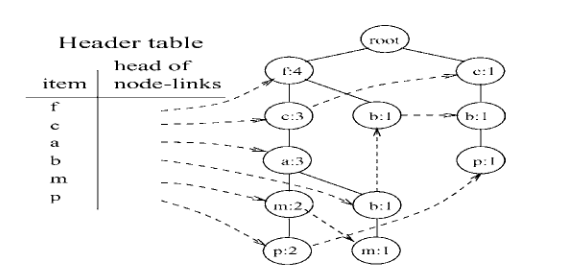
\includegraphics[scale=0.5]{fp-tree}
  \centering
  \caption{\textit{FP-tree}.}
  \label{fig:rbt}
\end{figure}

Analysis.\quad The FP-tree construction takes exactly two scans of the transaction database: The first scan collets the set of frequent items, and the second scan constructs the FP-tree. The cost of inserting a transaction $T$ into the FP-tree is $\mathcal{O}(freq(T))$, where $freq(T)$ is the set of frequent items in $T$.

The following \textit{lemmas} are necessary to proof that an \textit{FP-tree} is a compact and efficient data structure and encodes the same information as the original database i.e. it is sufficient scanning the \textit{FP-tree} to find the complete set of frequent itemsets of the database DB.

\begin{lemma}
  Given a transaction database DB and a support threshold $\xi$, the complete set of frequent item projections of transactions in the database can be derived from DB's FP-tree.
\end{lemma}

\begin{lemma}
  Given a transaction database DB and a support threshold $\xi$. Without considering the (null) root, the size of an FP-tree is bounded by $\sum_{T \in DB} |freq(T)|$, and the height of the tree is bounded by $\underset{T \in DB}{\max} \{|freq(T)|\}$, where $freq(T)$ is the frequent item projection of the transaction $T$.
\end{lemma}

\section{Mining frequent patterns using FP-tree}

This section describes how to explore the comptact information stored in the \textit{FP-tree}, develops the principles of frequent-pattern growth, and proposes a frequent-pattern growth algorithm, \textit{FP-growth}, for mining the complete set of frequent patterns using the \textit{FP-tree}.

\begin{corollary}\label{cor:pattern-growth}
  (Pattern growth). \quad Let $\alpha$ be a frequent itemset in DB, B be $\alpha$'s conditional pattern-base, and $\beta$ be an itemset in B. Then $\alpha \cup \beta$ is frequent in DB if and only if $\beta$ is frequent in B.
\end{corollary}

Collorary \ref{cor:pattern-growth} is derived from an extensive chain of properties, proofs and examples that are present in the original paper which I recommend reading.

Collorary \ref{cor:pattern-growth} states that mining can be performed by first identifying the set of frequent 1-itemsets in DB, and then for each frequent 1-itemset, constructing its conditional pattern-bases, and mining its set of frequent 1-itemsets in the conditional pattern-base, and so on. This indicates that the process of mining frequent patterns can be viewed as first mining frequent 1-itemset and then progressively growing each itemset by mining its conditional pattern-base, which can in turn be done similarly. By doing so, a frequent $k$-itemset mining problem is successfully transformed into a sequence of $k$ frequent 1-itemset mining problems via a set of conditional pattern-bases. Since mining is done by \textit{pattern growth}, there is no need to generate any candidate sets in the entire mining process.

\begin{algorithm}[H]
  \SetKwInOut{Input}{Input}
  \SetKwInOut{Output}{Output}
  \BlankLine
  \Input{A database DB, represented by FP-tree and a minimum support threshold $\xi$}
  \BlankLine
  \Output{The complete set of frequent patterns.}
  \BlankLine

  Procedure FP-growth($Tree$, $alpha$) \\
  \{ \\
    \If{$Tree$ contains a single prefix path}{
      let $P$ be the single prefix-path part of $Tree$\\
      let $Q$ be the multipath part with the top branching node replaced by a \textit{null} root\\
      \ForEach{combination(denoted as $\beta$) of the nodes in the path $P$}{
        generate pattern $\beta \cup \alpha$ with $support$ = \textit{minimum support of nodes in $\beta$}
      }
      let \code{freq\_pattern\_set(P)} be the set of patterns so generated
    }
    \Else{let $Q$ be $Tree$}
    \ForEach{item $a_i$ in $Q$}{
      generate pattern $\beta = a_i \cup \alpha$ with support = $a_i . support$\\
      construct \beta 's conditional pattern-base and then \beta 's conditional FP-tree $Tree_{\beta}$\\
      \If{$Tree = \emptyset$}{
        call \code{FP-growth($Tree_{\beta}$, $\beta$)} \\
      }
      let \code{freq\_pattern\_set(Q)} be the set of patterns so generated
    }
    return \code{freq\_pattern\_set(P)} $\cup$ \code{freq\_pattern\_set(Q)} $\cup$ (\code{freq\_pattern\_set(P)} $\times$  \code{freq\_pattern\_set(Q)}) \\
  \}
  \caption{FP-growth: Mining frequent patterns with \textit{FP-tree} by pattern fragment growth.}
  \label{scol}
\end{algorithm}

This algorithm is proven to be enough to find the complete set of frequent itemsets in transaction database DB \cite{han2000}. When the FP-tree contains a single prefix-path, the generation of the complete set of frequent patterns can be partitioned into three portions: the single prefix-path portion $P$, the multipath portion $Q$, and their combination, line (17). This is extensively explained in the original paper and it is an essencial optimization of the \textit{FP-growth} algorithm.

\section{Experimental evaluation and performance study}

\textit{FP-growth} is compared with the classical frequent pattern mining algorithm \textit{Apriori}, and an alternative database projection-based algorithm, \textit{TreeProjection}. The experiments are pursued on both synthetic and real data sets.

The first experiment (figure \ref{fig:compactness}) is to test the compactness of \textit{FP-trees}. They compared the sizes of the following structures.

\begin{itemize}
  \item \code{Alphabetical FP-tree}. It includes the space of all the links. However, in such an FP-tree,the alphabetical order of items are used instead of frequency descending order.
  \item \code{Ordered FP-tree}. Again, the size covers that of all links. In such an FP-tree, the items aresorted according to frequency descending order.
  \item \code{Transaction database}. Each item in a transaction is stored as an integer. It is simply thesum of occurrences of items in transactions.
  \item \code{Frequent transaction database}. That is the sub-database extracted from the original oneby removing all infrequent items.
\end{itemize}

\begin{figure}[H]
  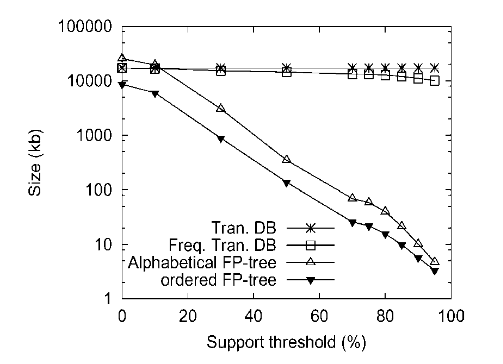
\includegraphics[scale=0.6]{fp-tree-compactness}
  \centering
  \caption{Compactness of \textit{FP-tree} over data set \textit{Connect-4}.}
  \label{fig:compactness}
\end{figure}

\newpage

The runtime of \textit{Apriori}, \textit{TreeProjection}, and \textit{FP-growth} on synthetic data set \code{T10.I4.D100K} as the support threshold decreases from $0.15\%$ to $0.01\%$ is shown in figure \ref{fig:runtime}. \textit{FP-growth} is faster than both \textit{Apriori} and \textit{TreProjection}.

\begin{figure}[H]
  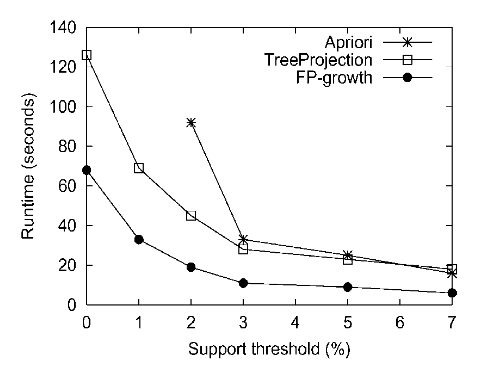
\includegraphics[scale=0.5]{fp-tree-runtime}
  \centering
  \caption{Scalability with threshold over sparse data set.}
  \label{fig:runtime}
\end{figure}

The advantages of \textit{FP-growth} over \textit{Apriori} becomes obvious when the dataset contains an abundant number of mixtures of short and long frequent patterns. The authors of the paper conducted several more experiments that can be found in the original paper.

\section{Conclusions}

The presented approach in the paper based on a comptact representation of the database, the \textit{frequent pattern tree (FP-tree)} and the developed mining algorithm based on a \textit{pattern growth} approach offers several advantages over other approaches: (1) highly comptact FP-tree which saves the costly database scans. (2) It applies a pattern growth method which avoids costly candidate generation and test by successively concatenating frequent 1-itemset found in the FP-trees. (3) It applies partitioning-based divide-and-conquer method which dramatically reduces the size of the subsequent conditional  pattern bases and conditional FP-tree.

The results of the tests performed show that \textit{FP-growth} outperforms the current candidate pattern generation-based algorithm, in both short and long patterns databases with a huge number of elements.

Since the publication of \textit{FP-growth} method for mining frequent patterns without candidate generation \cite{han2000}, there have been many subsequent studies on improvements of performance of frequent patterns based on the pattern-growth philosophy \cite{zhang2014}, as well as extension of the scope of the method to cover other kinds of pattern minin tasks \cite{li2012}.

%%%%%%%%%%%%%%%% BIBLIOGRAPHY %%%%%%%%%%%%%%%%%%%%%

\bibliographystyle{alpha}
\bibliography{refs}

\end{document}
